\section{Designdokumentation}
\subsection{Designklassediagram}
\begin{figure}[H]
            \centering
            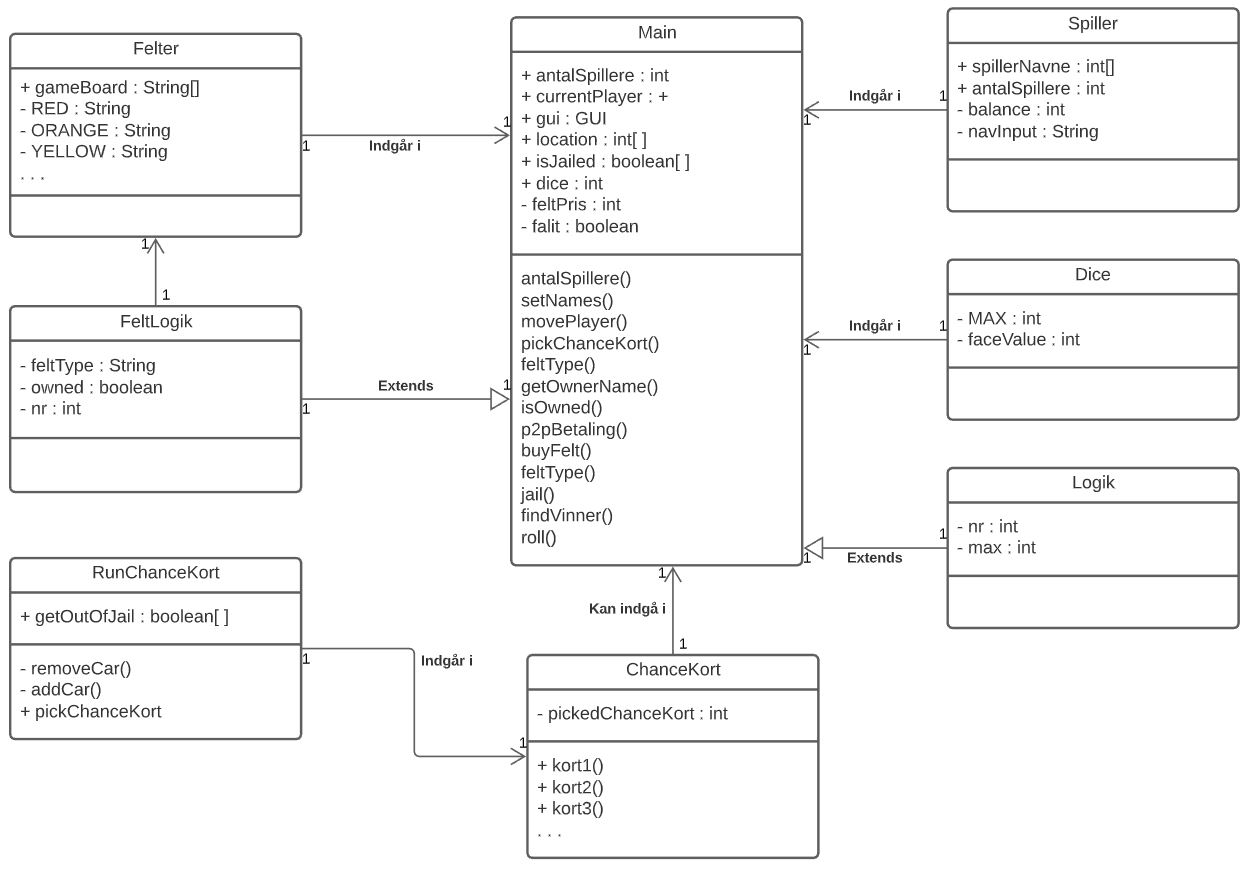
\includegraphics[width=14cm]{figures/designKlasseDiagram.JPG}
            \caption{Designklassediagram}
        \end{figure}

FORKLAR DESIGNKLASSEDIAGRAM og hvordan det hænger sammen.

Design-klassediagrammet benyttes i alt sin simpelhed til at give et  hurtigt og overordnet overblik over systemets klasser og hvordan de er relateret til hinanden.  Klassediagrammet viser hvilke metoder og attributter der tilhøre den enkelte klasse, samt hvilke klasser der er associeret med hinanden. 

Ud fra klassediagrammet kan det ses, at der er en "main" klasse, den klasse består af en længere række attributter som f.eks. antalSpillere, Gui, dice osv. Desuden er klassen tildelt samtlige metoder deriblandt, setName, movePlayer, feltType m.m. Main klassen er associeret med lige præcis 5 klasser, hvor netop Main indgår. Endvidere kan det ses at  klasserne FeltLogik og Logik er nedarvet af Main, hvad også kaldes subclass og superclass. 

Det bør evt. skrives noget på alle pilene
        
\subsection{Sekvensdiagram}
    \begin{figure}[H]
        \centering
        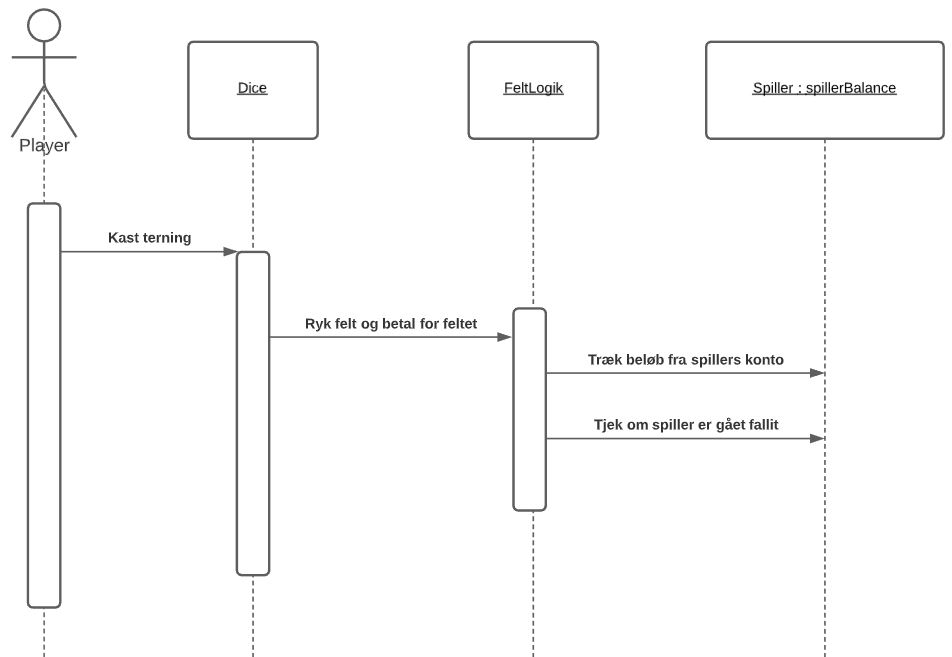
\includegraphics[width=15cm]{figures/systemSekvensDiagram.JPG}
        \caption{Sekvensdiagram}
        \emph{Sekvensdiagrammet illustrerer hvordan spillet virker som helhed}
    \end{figure}

\subsection{Brugergrænseflade}
